\begin{ejercicio}{1}
    Hallar los valores de \( n \) para los cuales \( C_n \) admite un matching perfecto. Adicionalmente, determinar para cada \( n \) el tamaño mínimo de un matching maximal de \( C_n \).
\end{ejercicio}
\begin{proof}

\end{proof}

\vspace{0.5cm}

\begin{ejercicio}{2}
    Probar que todo árbol tiene a lo sumo un matching perfecto.
\end{ejercicio}
\begin{proof}

\end{proof}

\vspace{0.5cm}

\begin{ejercicio}{3}
    Sea \( S \) el conjunto de vértices saturados por un matching \( M \) en un grafo \( G \). Probar que existe un matching máximo que también satura a todo \( S \). ¿Vale en general que cualquier otro matching máximo satura a \( S \) también?
\end{ejercicio}
\begin{proof}

\end{proof}

\vspace{0.5cm}

\begin{ejercicio}{4}
    Dos personas juegan un juego sobre un grafo \( G \), alternativamente eligiendo vértices distintos. El jugador 1 comienza eligiendo un vértice. Cada subsecuente elección debe ser adyacente a la anterior (del otro jugador). Así, a medida que avanza el juego, se sigue un camino. Pierde el jugador que no puede realizar ningún movimiento. Probar que el segundo jugador tiene una estrategia ganadora si \( G \) tiene un matching perfecto y que, en caso contrario, es el primer jugador quien la tiene.
\end{ejercicio}
\begin{proof}

\end{proof}

\vspace{0.5cm}

\begin{ejercicio}{5}
    Determinar si el siguiente grafo (con matching \( M \) en rojo) posee un matching perfecto, usando el algoritmo de caminos alternantes y blossoms.
    \begin{center}
        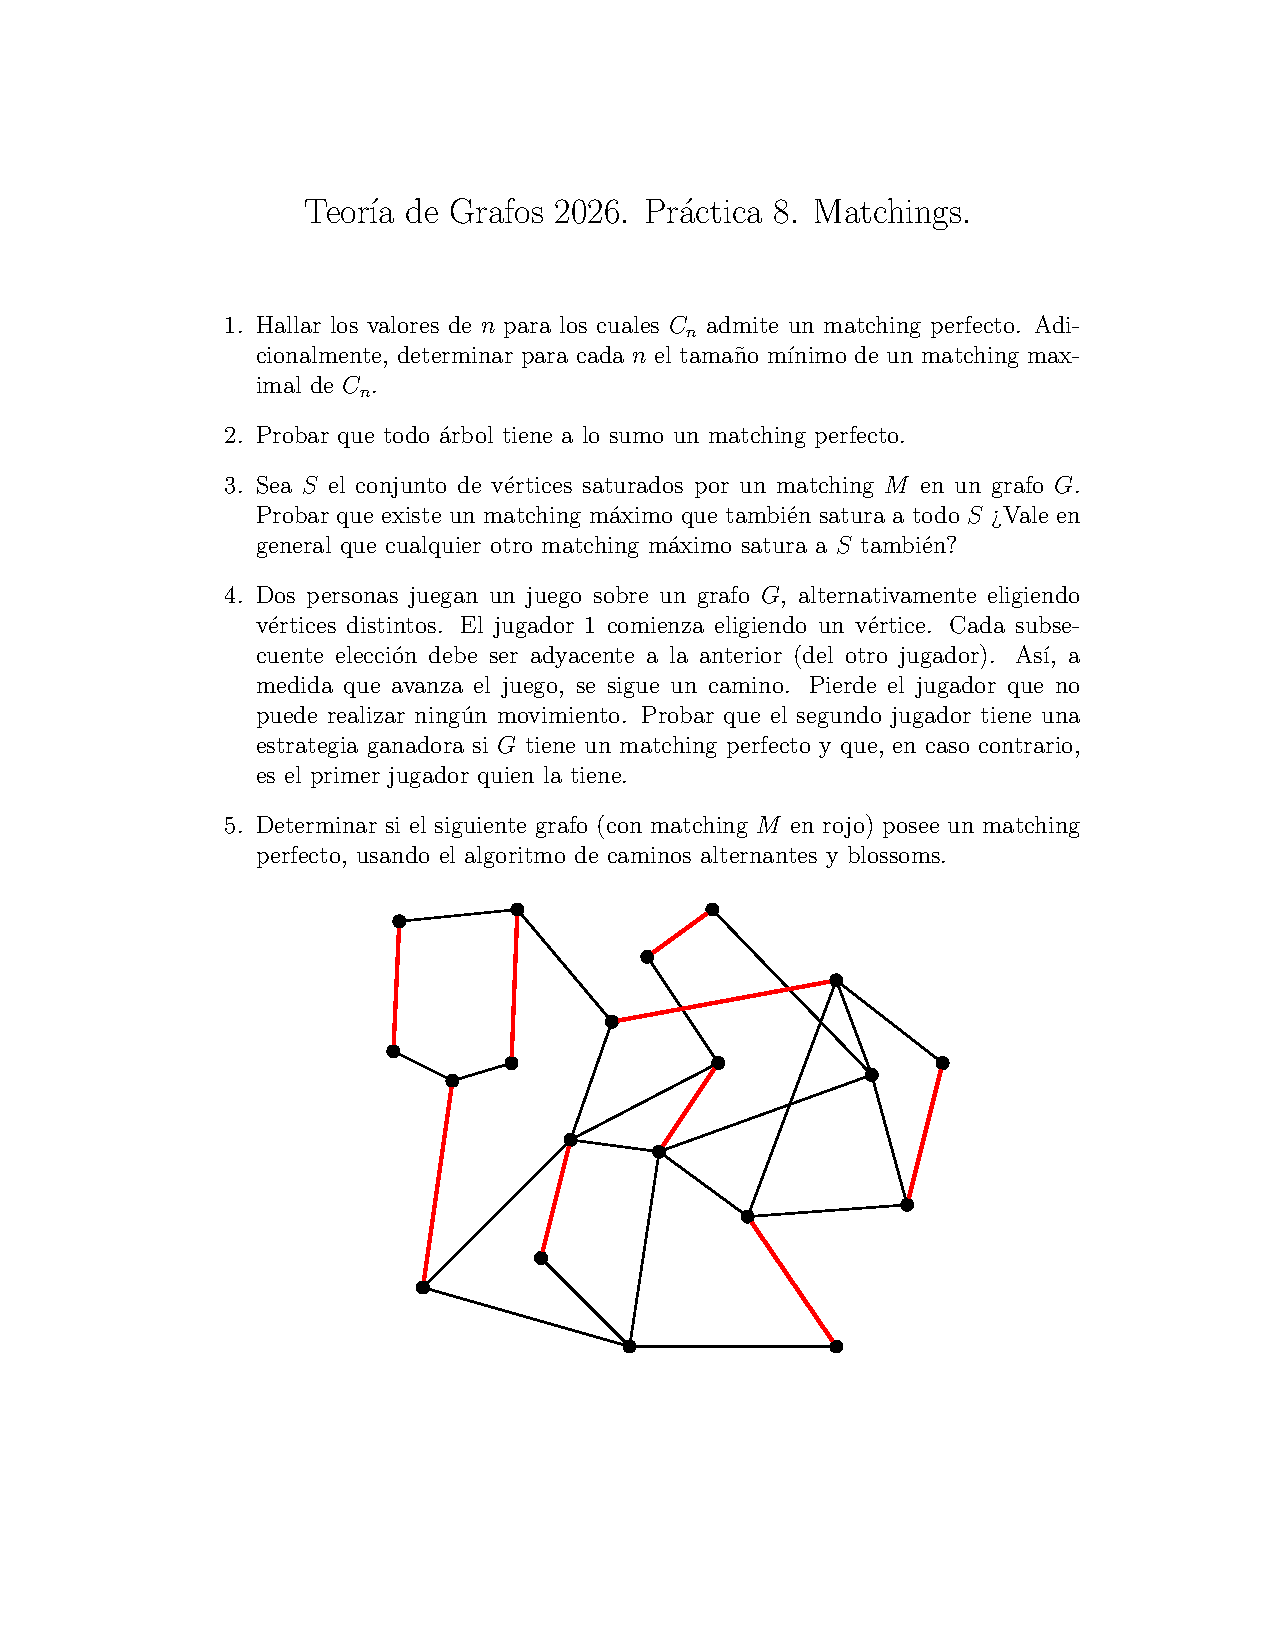
\includegraphics[page=1, trim=178pt 137pt 150pt 428pt, clip, width=0.55\linewidth]{p8/43_9_22112026042234.pdf}
    \end{center}
\end{ejercicio}
\begin{proof}

\end{proof}

\vspace{0.5cm}

\begin{ejercicio}{6}
    Encontrar un matching perfecto en el siguiente grafo, o dar una breve demostración de por qué no hay uno.
    \begin{center}
        \includegraphics[page=2, trim=164pt 508pt 142pt 149pt, clip, width=0.7\linewidth]{p8/43_9_22112026042234.pdf}
    \end{center}
\end{ejercicio}
\begin{proof}

\end{proof}

\vspace{0.5cm}

\begin{ejercicio}{7}
    Dado un conjunto \( S \) de vértices de un grafo, llamamos \( N(S) \) al conjunto de vértices que son adyacentes a al menos uno de \( S \) (en otras palabras, es la unión de las vecindades abiertas de los vértices de \( S \)). Probar que un grafo bipartito \( G \) posee un matching perfecto si y sólo si \( |N(S)| \geq |S| \) para todo subconjunto \( S \) de vértices. Encontrar un conjunto infinito de grafos no bipartitos que cumplen esta condición sin tener un matching perfecto.
\end{ejercicio}
\begin{proof}

\end{proof}

\vspace{0.5cm}

\begin{ejercicio}{8}
    Hallar un matching máximo para cada uno de los siguientes grafos bipartitos. Probar que la solución hallada es óptima exhibiendo un cubrimiento mínimo por vértices.
    \begin{center}
        \includegraphics[page=2, trim=92pt 260pt 114pt 467pt, clip, width=0.95\linewidth]{p8/43_9_22112026042234.pdf}
    \end{center}
\end{ejercicio}
\begin{proof}

\end{proof}

\vspace{0.5cm}

\begin{ejercicio}{9}
    Para cada uno de \( \alpha, \alpha', \beta, \beta' \), caracterizar a los grafos simples para los cuales el valor del parámetro es igual a \( 1 \).
\end{ejercicio}
\begin{proof}

\end{proof}

\vspace{0.5cm}

\begin{ejercicio}{10}
    Sea \( G \) un grafo con pesos en sus aristas. Un matching \( M \) de \( G \) es de peso máximo si maximiza la suma de los pesos de sus aristas. Usando pesos no negativos para las aristas, construir un grafo de cuatro vértices tal que su matching de peso máximo no es un matching de tamaño máximo.
\end{ejercicio}
\begin{proof}

\end{proof}

\vspace{0.5cm}

\begin{ejercicio}{11}
    Aplicar el algoritmo húngaro para hallar un matching de peso máximo en el siguiente grafo.
    \begin{center}
        \includegraphics[page=3, trim=238pt 420pt 205pt 144pt, clip, width=0.4\linewidth]{p8/43_9_22112026042234.pdf}
    \end{center}
\end{ejercicio}
\begin{proof}

\end{proof}
